\section{PDCA}\label{PDCASection}
Il PDCA, noto anche come Ciclo di Deming, è un modello studiato per il miglioramento continuo della qualità dei processi istanziati. Attraverso questa strategia il gruppo di lavoro cerca di ottimizzare l'uso delle risorse durante l'intero ciclo di vita del prodotto puntando ad un risultato di qualità. Il nome di fatto è un acronimo qui scomposto:
\begin{center}
	\item \textbf{P}lan-\textbf{D}o-\textbf{C}heck-\textbf{A}ct
\end{center}
Questo modello si suddivide in quattro iterazioni:
\begin{itemize}
	\item \textbf{Plan}: fase di pianificazione, nella quale vengono stabiliti obbiettivi metrici da raggiungere e processi da utilizzare, in base ai risultati attesi;
	\item \textbf{Do}: in questa fase vengono attuate le soluzioni ed i piani precedentemente definiti, eseguendo il programma. Inoltre, vengono raccolti i dati per la fase successiva;
	\item \textbf{Check}: test e controllo, si studiano i risultati ottenuti dall'esecuzione del programma (rilevati nel "DO") confrontandoli con i risultati attesi (trovati nel "PLAN"); 
	\item \textbf{Act}: si agisce sulla base dei risultati ottenuti e dei risultati attesi, al fine di migliorare i processi o il prodotto, non conformi alle attese. Finita questa fase, si procede con una nuova iterazione ripartendo dalla fase di Plan, potendo definire obbiettivi più stringenti laddove rispettati nell'iterazione appena terminata.
\end{itemize}
In sostanza il PDCA è un modello in cui, una volta soddisfatti gli obiettivi inizialmente pianificati, vengono fissati nuovi obiettivi da raggiungere per innalzare il livello di qualità.

\begin{figure}[H]
\centering
	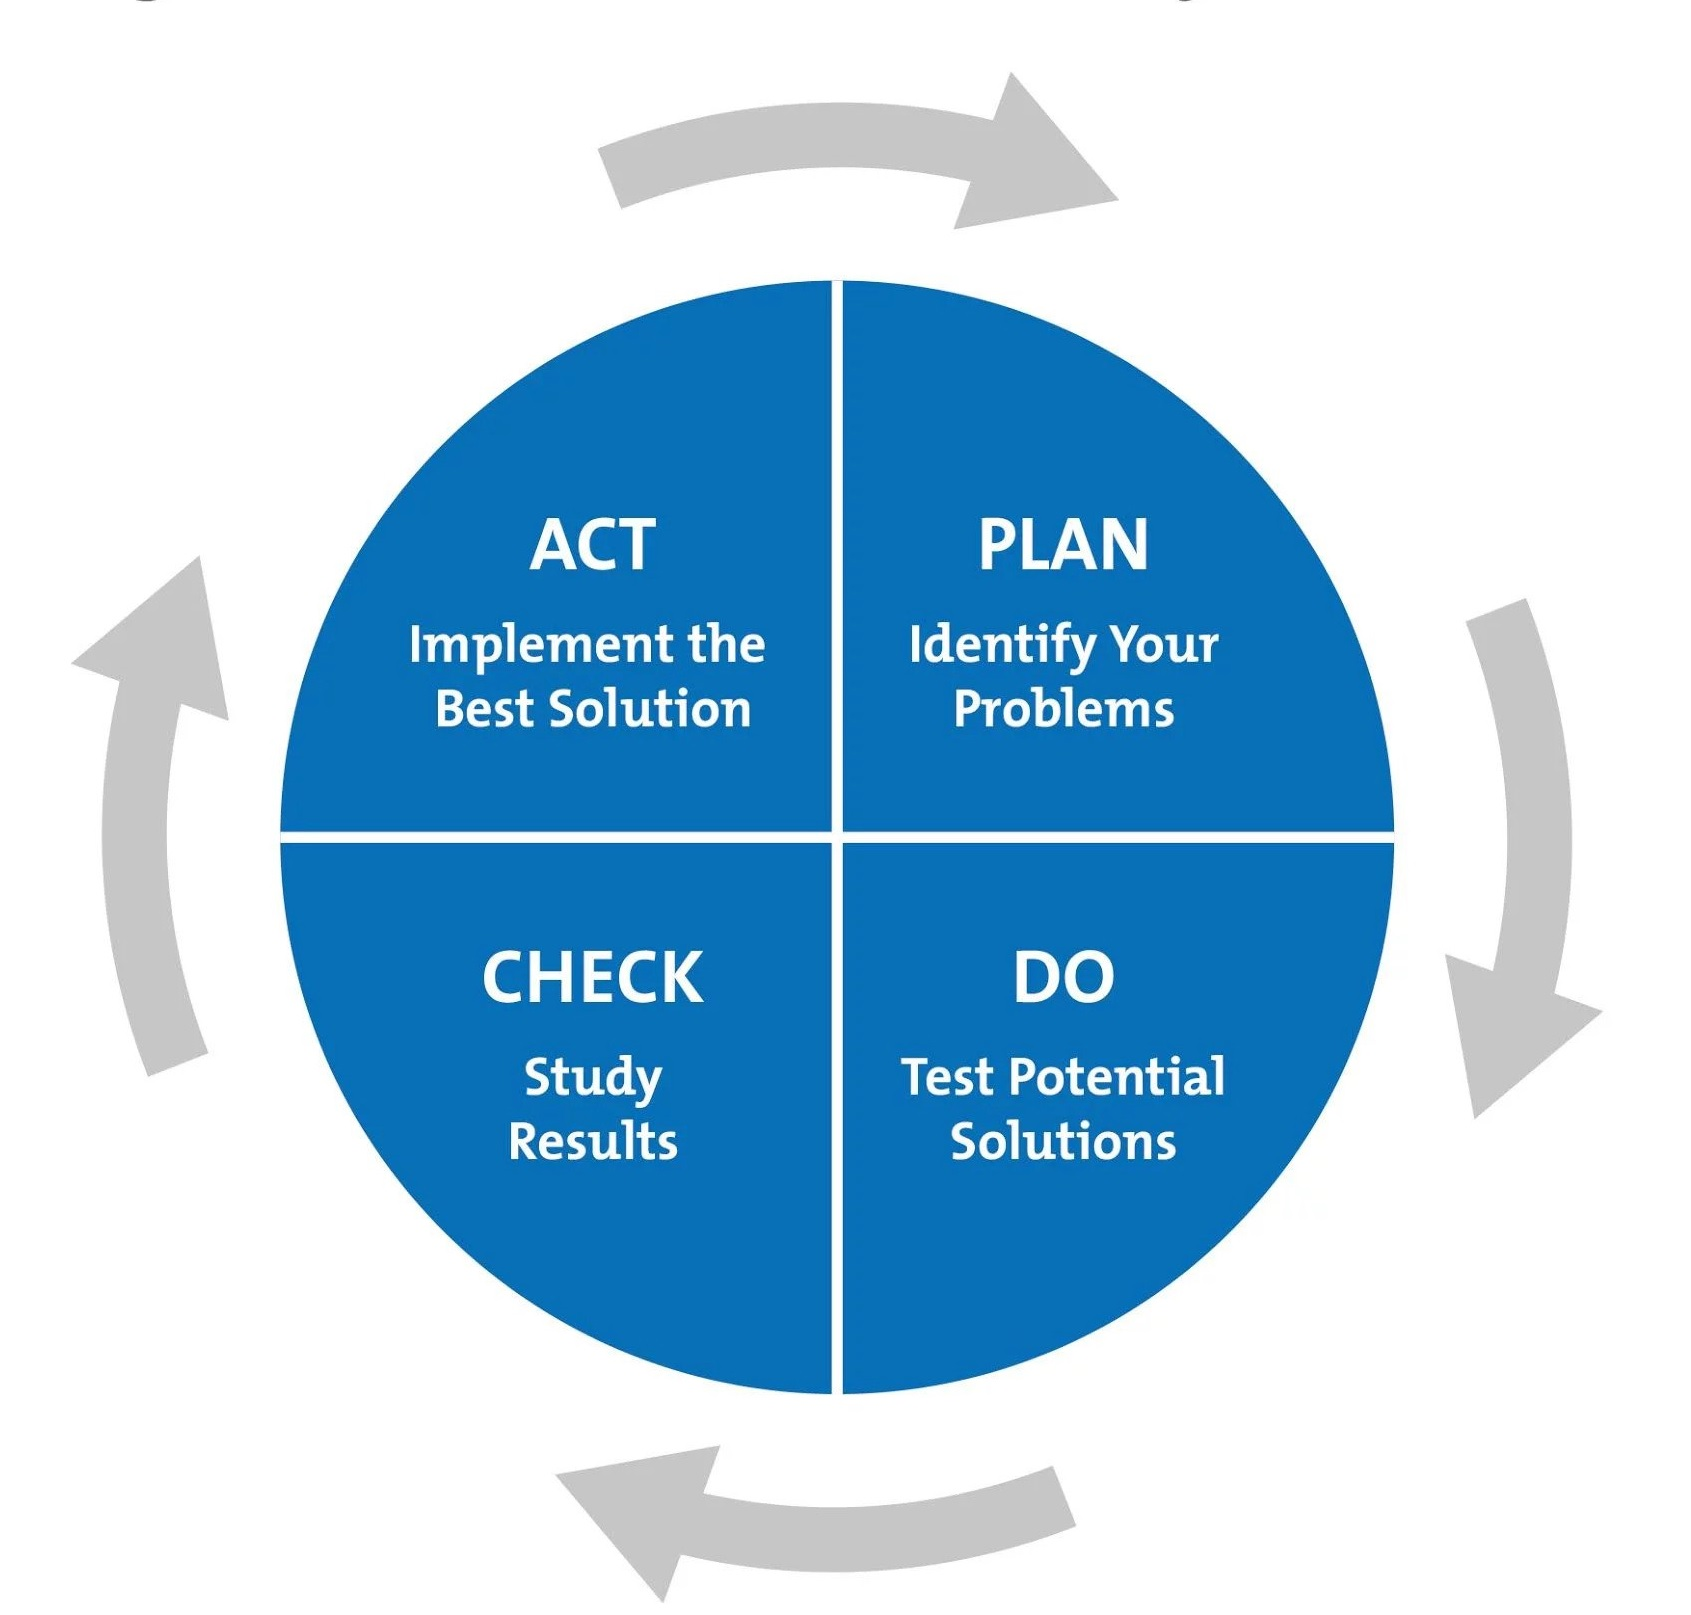
\includegraphics[width=0.4\linewidth]{./images/pdca.jpg}
	\caption{Modello PDCA. Immagine dal sito web \url{https://www.mindtools.com/pages/article/newPPM_89.htm}}
	\label{pdca}
\end{figure} 

 